\subsection{Filterung der Zustandsgrößen}
In der Regel werden Sensoren von Störungen unterschiedlichster Art beeinflusst. Deshalb werden in diesem Abschnitt verschiedene Ansätze vorgestellt um die Zustandsgrößen $\varphi$, $\dot{\varphi}$ und $\dot{\psi}$ zu filtern. 

\subsubsection{Ansätze zur Filterung von $\varphi$}
Der Ausfallwinkel $\varphi$ kann wie bereits vorgestellt aus den Beschleunigungswerten geschätzt werden. Alternativ kann die aktuelle Winkelgeschwindigkeit $\dot{\varphi}$, welche mit Hilfe der Gyroscope gemessen wird, integriert werden. Beide Ansätze werden von unterschiedlichen Rauschsignale beeinflusst. Die Beschleunigungssensoren reagieren empfindlich auf hochfrequente Signale und verstärken diese. Dadurch sind die Winkelschätzungen, welche auf diesen Messwerten beruhen, von hochfrequenten Rauschsignalen betroffen. 
Die Gyroscope-Werte sind trotz der Justierung mit einem Offset behaftet. Durch die Integration dieses konstanten Signales ensteht ein tieffrequentes Rauschsignale, welches oftmals als Drift bezeichnet wird. 
Deshalb werden im Anschluss das Komplementär- und Kalman-Filter vorgestellt, wobei es sich um Methoden der Datenfusion handelt.

\subsubsubsection{Komplementär-Filter für $\varphi$}
Wie bereits erläutert liefert die Winkelschätzung aus den Beschleunigungswerten das verrauschte Signal $\varphi^A$ und die Integration der Gyroscopewerte $\varphi^G$.
\begin{equation}
\begin{split}
\varphi^A(s) &= \varphi(s) + x^A(s) \\
\varphi^G(s) &= \frac{1}{s} \cdot (\dot{\varphi} + \dot{x^G}) 
\end{split}
\end{equation}

Angenommen, dass $\varphi^A$ mit Hilfe eines Tiefpass und $\varphi^G$ mit Hilfe eines Hochpass gefiltert werden, so ergibt sich das folgende Blockschaltbild.

\begin{figure}[!h]
\includegraphics[scale=0.5,trim={0 3cm 0 4cm},clip]{img/Komp_CuBa_1D}
\end{figure}

Nach dem Blockschaltbild ergibt sich im Bildbereich der folgende Zusammenhang.

\begin{equation}
\label{comp_bildbereich_eq}
\begin{split}
\varphi^C(s) &= \frac{1}{1 + \tau_1 \cdot s} \cdot \varphi^A(s) + \frac{\tau_2 \cdot s}{1 + \tau_2 \cdot s} \cdot \frac{1}{s} \cdot \dot{\varphi}^G(s) \\
&= \frac{1}{1 + \tau_1 \cdot s} \cdot [\varphi(s) + x^A(s)] + \frac{\tau_2 \cdot s}{1 + \tau_2 \cdot s} \cdot [\varphi(s) + x^G(s)]
\end{split}
\end{equation}

Als erste Entwurfsbedinung müssen die beiden Zeikonstanten $\tau_1$ und $\tau_2$ so gewählt werden, dass die Rauschanteile $x^A$ und $x^G$ verschwinden. Falls dies gegeben ist, lässt sich (\ref{comp_bildbereich_eq}) vereinfachen.
\begin{equation}
\begin{split}
\varphi^C(s) &= \frac{1}{1 + \tau_1 \cdot s} \cdot \varphi(s) + \frac{\tau_2 \cdot s}{1 + \tau_2 \cdot s} \cdot \varphi(s) \\
&= \varphi(s) \cdot (\frac{1}{1 + \tau_1 \cdot s} + \frac{\tau_2 \cdot s}{1 + \tau_2 \cdot s})
\end{split}
\end{equation}
Falls die beiden Zeitkonsanten, unter Einhaltung der ersten Bedingung, gleichgesetzt werden können, ergibt sich die folgende Übertragungsfunktion für das Komplementär-Filter.
\begin{equation}
\tau = \tau_1 = \tau_2
\end{equation}
\begin{equation}
\varphi^C(s) = \varphi(s) \cdot (\frac{1}{1 + \tau \cdot s} + \frac{\tau \cdot s}{1 + \tau \cdot s}) = \varphi(s)
\end{equation}

Um die gennanten Bedinungen zu erfüllen muss eine Spektralanalyse der Rauschsignale durchgeführt werden. Welche verwendet wird um die Grenzfrequenzen des Hoch- und Tiefpassfilters festzulegen. Anschließend wird geprüft ob diese gleichgesetzt werden können.

Die Berechnung des Komplementär-Filters findet auf einem Digitalrechner statt. Somit muss (\ref{comp_bildbereich_eq}) in eine diskrete Berechnungsvorschrift transformiert werden. Hierfür können das Hochpassfilter und der Integrator zu einem Tiefpass zusammengeführt werden.
\begin{equation}
\label{Comp_Bild_eq}
\varphi^C(s) = \frac{1}{1 + \tau \cdot s} \cdot \varphi^A(s) + \frac{\tau}{1 + \tau \cdot s} \cdot \dot{\varphi}^G(s)
\end{equation}

Mit Hilfe der Backward-Euler-Tranformation kann (\ref{Comp_Bild_eq}) als Z-Transformierte dargestellt werden.
\begin{equation}
s = \frac{1 - z^{-1}}{T}
\end{equation}
\begin{equation}
\begin{split}
\varphi^C(z) & = \frac{1}{1 + \tau \cdot \frac{1 - z^{-1}}{T} } \cdot \varphi^A(z) + \frac{\tau}{1 + \tau \cdot \frac{1 - z^{-1}}{T}} = \\
& = \frac{T}{T + \tau - \tau \cdot z^{-1}} \cdot \varphi^A(z) + \frac{\tau \cdot T}{T + \tau - \tau \cdot z^{-1}} \cdot \dot{\varphi}^G(z)
\end{split}
\end{equation}

\begin{equation}
\begin{split}
(T + \tau - \tau \cdot z^{-1}) \cdot \varphi^C(z) = T \cdot \varphi^A(z) + \tau \cdot T \cdot \dot{\varphi}^G(z)
\end{split}
\end{equation}

\begin{equation}
(T + \tau) \cdot \varphi^C(z) = \tau \cdot [\varphi^C(z) \cdot z^{-1}  + T \cdot \dot{\varphi}^G(z)] + T \cdot \varphi^A(z)
\end{equation}

\begin{equation}
\begin{split}
\varphi^C(z) & = \frac{\tau}{\tau + T}[\varphi^C(z) \cdot z^{-1}  + T \cdot \dot{\varphi}^G(z)] + \frac{T}{T + \tau} \varphi^A(z) \\
& = \frac{\tau}{\tau + T}[\varphi^C(z) \cdot z^{-1}  + T \cdot \dot{\varphi}^G(z)] + (1 - \frac{\tau}{T + \tau}) \varphi^A(z)
\end{split}
\end{equation}

Durch die Substitution $\alpha = \frac{\tau}{\tau + T}$ kann weiter vereinfacht werden. 

\begin{equation}
\varphi^C(z)  = \alpha[\varphi^C(z) \cdot z^{-1}  + T \cdot \dot{\varphi}^G(z)] + (1 - \alpha) \varphi^A(z)
\end{equation}
\begin{equation}
\varphi^C_n = \alpha(\varphi^C_{n-1}  + T \cdot \dot{\varphi}^G_n) + (1 - \alpha) \varphi^A_n
\end{equation}

\subsubsubsection{Kalman-Filter für $\varphi$}
Das Kalman-Filter beruht auf dem Prinzip der Zustandsschätzung. Diese Schätzung erfolgt mittels der Messwerte aus Gyroskopen, Beschleunigungssensoren und der darauf folgenden Winkelschätzung. Hierbei greift der Algorithmus auf Methoden der Wahrscheinlichkeitsrechnung zurück. Ist die Varianz eines Messfehlers gegeben, so kann eine Schätzung des tatsächlichen Zustandes vorgenommen werden.
In diesem Fall wird mit den linearisierten Bewegungsgleichungen gearbeitet. Dadurch kann das gewöhnliche Kalman-Filter verwendet werden. Für nichtlineare Systeme müssen unterschiedliche Filteralgorithmen, wie beispielsweise das Extended-Kalman-Filter, verwendet werden.


\begin{table}[h!]
\centering
\begin{tabularx}{0.9\textwidth}{|c|c|}
\hline
 \textbf{Bezeichnung}  	& \textbf{Erkärung} \\ \hline
 $\boldsymbol{x}^*_n$	&	Systemzustände \\ \hline
 $\hat{\boldsymbol{x}}_n$ & Geschätzte Systemzustände \\ \hline 
 $\boldsymbol{u}_n$		& 	Messbare Eingangsgrößen  \\ \hline
 $\boldsymbol{v}_n$		&	Störgrößen \\ \hline
 $\boldsymbol{A}_d$ 	& 	Systemmatrix, welche den Systemzustand $\hat{\boldsymbol{x}}_n$  \\  & auf den folgenden Zeitschritt abbildet. \\ \hline
 $\boldsymbol{B}_d$		&	Eingangsmatrix \\ \hline
 $\boldsymbol{C}_d$		&	Ausgangsmatrix \\ \hline
 $\boldsymbol{P}^*_n$	&	Kovarianzmatrix von $\boldsymbol{x}^*_n$. Legt die Sicherheit der Schätzung fest. \\ \hline
 $\hat{\boldsymbol{P}}_n$ & Filterkovarianzmatrix von $\hat{\boldsymbol{x}}_n$. Gibt die Gewichtung der Messwerte an. \\ \hline
 $\boldsymbol{Q}_n$		&	Kovarianzmatrix des Systemrauschens \\ \hline
 $\boldsymbol{R}_n$		& 	Kovarianzmatrix des Messrauschens \\ \hline
\end{tabularx}
\end{table}

Die Berechnung des Kalman-Filters verläuft in zwei Schritten, welche in insgesamt fünf Teile gegliedert ist. Zuerst wird der Prädikationsschritt durchgeführt, hierbei wird der Prädikationsschätzwert $\boldsymbol{x}^*_{n+1}$ berechnet, welcher den Systemzustand im folgenden Zeitschritt darstellt. Zusätzlich wird die Prädikationskovarianzmatrix $\boldsymbol{P}^*_{n+1}$ berechnet, welche angibt wie sicher die Vorhersage im Verhältnis zu dem wahren Systemzustand ist.
Im zweiten Abschnitt, der s.g. Korrektur- bzw. Filterschritt, wird die Vorhersage mit Hilfe der neuen Messwerte korrigiert. Hierfür wird zuerst die Verstärkungsmatrix $\boldsymbol{K_{n+1}}$ berechnet, welche den Rückkopplungsfaktor der Messwerte wiedergibt. Im Anschluss wird der Endschätzwertes des Systemzustandes mit Hilfe des ersten Prädikationswertes $\boldsymbol{x}^*_{n+1}$ und der Verstärkungsmatrix $\boldsymbol{K}_{n+1}$ bestimmt. Zuletzt wird die Varianz des geschätzten Systemzustandes $\hat{\boldsymbol{P}}_{n+1}$ berechnet.

\begin{enumerate}
	\item \textbf{Prädikationsschätzwert}
	\newline
	Der Systemzustand zum Zeitpunkt $n$ ist beschreibbar durch die zeitdiskrete, lineare, stochastische Differenzengleichung
	\begin{equation}
	\boldsymbol{x}^*_{n+1} = \boldsymbol{A}_d \cdot \boldsymbol{\hat{x}}_n + \boldsymbol{B} \cdot \boldsymbol{u}_n + \boldsymbol{v}_n
	\end{equation}
	Die Systemmatrix $\boldsymbol{A}$ bildet den Systemzustand $\boldsymbol{\hat{x}}$ von Zeitschritt $n$ auf den folgenden Zeitschritt $n+1$ ab. Die Eingangsgrößen $\boldsymbol{u}_n$ werden durch die Matrix $\boldsymbol{B}$ auf den Systemzustand $\boldsymbol{x}^*_{n+1}$ abgebildet. Das Rasuchen bzw. die äußeren Störeinflüsse werden durch den additiven Term $\boldsymbol{v}_n$ repräsentiert.
	\item \textbf{Prädikationskovarianzmatrix}
	\newline
	Die Kovarianzmatrix $\boldsymbol{P}^*_{n+1}$ gibt an, wie sicher die Prädikation im Verhältnis zu dem wahren Systemzustand ist.
	\begin{equation}
	\boldsymbol{P}^*_{n+1} = \boldsymbol{A} \cdot \boldsymbol{\hat{P}}_n \cdot \boldsymbol{A}^T + \boldsymbol{Q}_n
	\end{equation}
	\item \textbf{Verstärkungsmatrix} \newline
	Die Verstärkungsmatrix $\boldsymbol{K}_{n+1}$ wird für die Korrektur der Vorhersage verwendet. Sie bestimmt, mit welcher Verstärkung der Messvektor rückgekoppelt wird.
	\begin{equation}
	\boldsymbol{K}_{n+1} = (\boldsymbol{P}^*_{n+1} \cdot \boldsymbol{C}^T)(\boldsymbol{C} \cdot \boldsymbol{P}^*_{n+1} \cdot \boldsymbol{C}^T + \boldsymbol{R}_{n+1})^{-1}
	\end{equation}
	\item \textbf{Filterschätzwert}
	Mit Hilfe der Verstärkungsmatrix $\boldsymbol{K}_{n+1}$ und des Prädikationswertes $\boldsymbol{x}^*_{n+1}$ wird der finale Schätzwert des Systemzustandes zu dem Zeitpunkt $n+1$ bestimmt.
	\begin{equation}
	\boldsymbol{\hat{x}}_{n+1} = \boldsymbol{x}^*_{n+1} + \boldsymbol{K}_{n+1}(\boldsymbol{y}_{n+1} - \boldsymbol{C} \cdot \boldsymbol{x}^*_{n+1})
	\end{equation}
	\item \textbf{Filterkovarianzmatrix}
	Im letzten Schritt wird die Varianz des geschätzten Systemzustandes berechnet, welche die Gewichtung der Messwerte im weiteren Verlauf der Berechnung beschreibt.
	\begin{equation}
	\boldsymbol{\hat{P}}_{n+1} = \boldsymbol{P}^*_{n+1} - \boldsymbol{K}_{n+1} \cdot \boldsymbol{C} \cdot \boldsymbol{P}^*_{n+1}
	\end{equation}
\end{enumerate}

\subsubsubsection*{Anwendung des Kalman-Filters}
Um die zuvor angesprochenen Nachteile der einzelnen Sensoren auszugleichen, wird nun die Umsetzung eines Kalman-Filters zur Sensorfusion vorgestellt.

Das Kalman-Filter fusioniert den Ausfallwinkel $\varphi_{Acc}$ aus der Winkelschätzung mit der Winkeländerung $\Delta \varphi_{Gyr}$, welche durch Integration der Gyroskopwerte gewonnen wurde. Daraus ergibt sich der gefilterte Winkel $\hat{\varphi}_n$. Dieser gefilterte Zustandswert wird für die Berechnung des Regelkreises verwendet.

Als absolute Eingangsgrößen stehen hier zum einen die Winkelschätzung $\varphi_{Acc}$ und die Winkeländerung $\Delta \varphi_{Gyr}$ zur Verfügung. Somit kann das fehlerbehaftete Teilsystem durch folgende Gleichungen beschrieben werden, wobei $v_{Gyr,n}$ $w_{Acc,n}$ die störbehafteten Additionstherme darstellen.

\begin{equation}
\varphi_{n+1} = \varphi_{n} + \Delta \varphi_{Gyr,n} + v_{Gyr,n}
\end{equation}
\begin{equation}
\varphi_{Acc,n} = \varphi_n + w_{Acc,n}
\end{equation}

\begin{figure}[!h]
\centering
\includegraphics[width=0.8\linewidth, trim={0 3.5cm 0 3.5cm},clip]{img/kalman_phi_overview}
\caption{Übersicht Kalman-Filter, Quelle: eigene Darstellung}
\end{figure}

Die bereits vorgestellten Berechnungsschritte können nun auf den spezifischen Anwendungsfall angepasst werden. Da lediglich eine einzelne Zustandsgröße berechnet wird, werden anstelle von Vektoren und Matrizen skalare Größen verwendet.

\begin{enumerate}
\item \textbf{Prädikationsschätzwert}
\begin{equation}
\varphi^*_{n+1} = \hat{\varphi}_n + \Delta \varphi_{Gyr,n}
\end{equation}
\item \textbf{Prädikationsvarianz}
\begin{equation}
P^*_{n+1} = \hat{P}_{n+1} + \sigma^2(\Delta \varphi_{Gyr,n})
\end{equation}
\item \textbf{Verstärkungsfaktor}
\begin{equation}
K_{n+1} = \frac{P^*_{n+1}}{P*_{n+1} + \sigma^2(\varphi_{Acc,n}}
\end{equation}
\item \textbf{Filterschätzwert}
\begin{equation}
\hat{\varphi}_{n+1} = \varphi^*_{n+1} + K_{n+1} \cdot (\varphi_{Acc,n} - \varphi^*_{n+1})
\end{equation}
\item \textbf{Filtervarianz}
\begin{equation}
\hat{P}_{n+1} = (1-K_{n+1}) \cdot P^*_{n+1}
\end{equation}
\end{enumerate}

\subsubsubsection{Vergleich der Filter}
Um einen ersten Eindruck über die Qualität der Filter zu erhalten wird die Würfelseite als gewöhnliches Pendel aufgebaut und in Schwingung versetzt. Anschließend werden die Sensorwerte ausgewertet und die beiden Filter berechnet. 

\begin{figure}[h!]
\centering
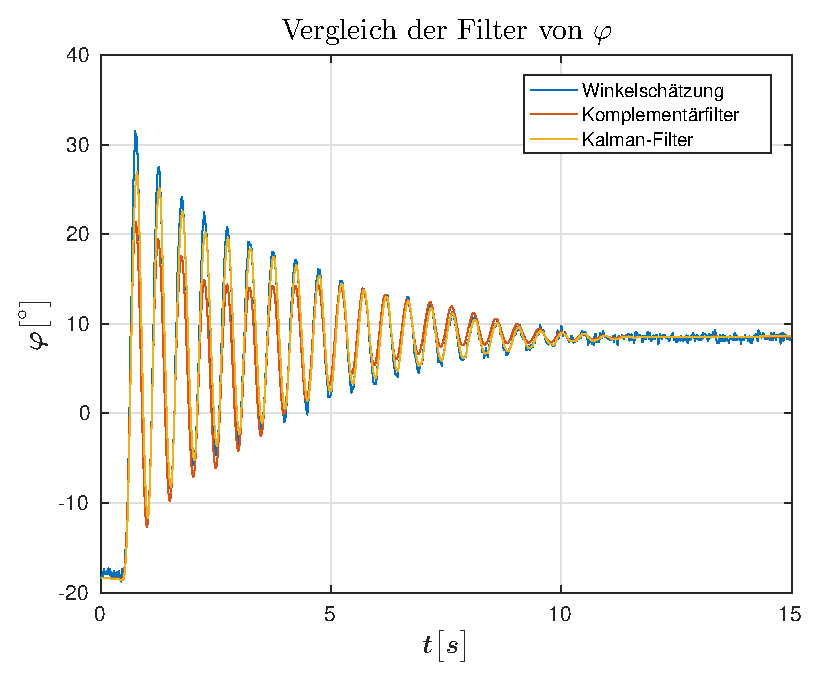
\includegraphics[width=0.5\linewidth]{img/filtervergleich_phi}
\caption{Vergleich der Filter für $\varphi$, Quelle: eigene Darstellung}
\end{figure}

Aus dem Verlauf der Signale lässt sich erkennen, dass die beiden Filter zu einer Glättung führen. Dennoch unterscheiden sich die Amplituden der drei Signale stark voneinander. Allerdings lassen sich diese Verläufe ohne ein Referenzsignal nicht weiter beurteilen. Somit kann eine endgültige Bewertung der Filter erst an Hand der Güte des geschlossenen Regelkreises getroffen werden.

\subsubsection{Ansätze zur Filterung von $\dot{\varphi}$}
Um die Winkelgeschwindigkeit $\dot{\varphi}$ zu ermitteln wird ebenfalls ein Kalman-Filter eingesetzt.
 
\begin{figure}[H]
\centering
\includegraphics[width=0.8\linewidth, trim={0 3.7cm 0 3.7cm},clip]{kalman_phi__d_overview}
\vspace*{-\baselineskip}
\end{figure}

In diesem Fall werden als Eingangsignale der Messwert des Gyroscopes $\dot{\varphi}_{Gyr}$ und integrierte Winkelbeschleunigung $\dot{\varphi}_{Acc}$ verwendet. Somit kann das fehlerbehaftete Teilsystem in seiner Dynamik durch folgende Gleichungen beschrieben werden, wobei die Störanteile der Beschleunigungssensoren und Gyroscope durch $v_{Acc,n}$ bzw. $w_{Gyr,n}$ dargestellt werden.
\begin{equation}
\dot{\varphi}_{n+1} = \dot{\varphi}_n + \Delta \dot{\varphi}_{Acc,n} + v_{Acc,n}
\end{equation}
\begin{equation}
\dot{\varphi}_{Gyr,n} = \dot{\varphi}_n + w_{Gyr,n}
\end{equation}
Die Zustandsschätzung verläuft analog zu dem bereits vorgestellten Verfahren.
\begin{enumerate}
\item \textbf{Prädikationsschätzwert}
\begin{equation}
\dot{\varphi}^*_{n+1} = \hat{\dot{\varphi}}_n + \Delta \dot{\varphi}_{Acc,n}
\end{equation}
\item \textbf{Prädikationsvarianz}
\begin{equation}
P^*_{n+1} = \hat{P}_{n+1} + \sigma^2(\Delta \dot{\varphi}_{Acc,n})
\end{equation}
\item \textbf{Verstärkungsfaktor}
\begin{equation}
K_{n+1} = \frac{P^*_{n+1}}{P*_{n+1} + \sigma^2(\dot{\varphi}_{Gyrs,n}}
\end{equation}
\item \textbf{Filterschätzwert}
\begin{equation}
\hat{\dot{\varphi}}_{n+1} = \dot{\varphi}^*_{n+1} + K_{n+1} \cdot (\dot{\varphi}_{Gyr,n} - \dot{\varphi}^*_{n+1})
\end{equation}
\item \textbf{Filtervarianz}
\begin{equation}
\hat{P}_{n+1} = (1-K_{n+1}) \cdot P^*_{n+1}
\end{equation}
\end{enumerate}
Die nächste Abbildung zeigt den Verlauf der Gyroscopewerte und des Kalman-Filters bei dem Versuch aus dem vorherigen Abschnitt.
\begin{figure}[!h]
\centering
\includegraphics[width=0.5\linewidth]{img/filtervergleich_phi__d}
\caption{Verlauf des Filters für $\dot{\varphi}$, Quelle: eigene Darstellung}
\end{figure}
Hier sind nur marginale Unterschiede zwischen den Amplituden zu erkennen. Ebenso wie die Filter für $\varphi$ muss die letzendliche Filtergüte am geschlossenen Regelkreis näher untersucht werden.

\newpage
\subsubsection{Ansätze zur Filterung von $\dot{\psi}$}
Die Winkelgeschwindigkeit $\dot{\psi}$ des Motors wird als analoges Signal von einem 12-Bit AD-Wandler ausgewertet. Diese Messwerte sind ebenfalls von hochfrequenten Störeinflüssen betroffen und müssen somit geglättet werden. Hierfür werden digitale Tiefpassfilter verwendet, welche in Form eines gleitenden Mittelwertes implementiert. Dieser Mittelwet wird über die letzen $N$ Messwerte gebildet. 

\begin{equation}
y_n = \frac{1}{N}\sum^{N-1}_{k=0} x_{n-k}
\end{equation}

Die Glättung des Filters nimmt mit der Anazhl der verwendeten Werte $N$ zu, allerdings wird das Filter damit auch träger. Somit muss ein Kompromis zwischen Verzögerung und Glättung gefunden werden. Die folgende Abbildung zeigt den Vergleich der nicht gefilterten Werte aus dem Versuch zur Bestimmung des Reibwertes $C_{\psi}$ und verschiedenen Mittelwert-Filtern. 

\begin{figure}[!h]
\centering
\includegraphics[width=0.6\linewidth]{img/filtervergleich_psi__d}
\end{figure}

Der Verlauf zeigt deutlich die Glättung des Signales. Außerdem ist keine signifikante Verzögerung durch die verschiedenen Filter ersichtlich. Allerdings ist zu erwarten, dass der Motor ein Eingangssignal mit höheren Frequenzanteilen erzeugt, sobald der Regelkreis geschlossen wird. Somit entsteht auch eine stärkere Verzögerung durch die Tiefpassfilter. Deshalb kann die optimale Konfiguration des Mittelwert-Filters erst an der realen Regelstrecke ermittelt werden.